% ------------ begin cheatsheet
\documentclass[a4paper]{article}
\usepackage[a4paper,margin=0.05in]{geometry}
\usepackage{multicol}

\usepackage{amsmath, amssymb}
\usepackage[inline]{enumitem}
\usepackage{graphicx}

\usepackage{ulem}
\usepackage{makecell}

% horizontal list
\newlist{hlist}{enumerate*}{1}
\setlist[hlist]{label={}, afterlabel={}, itemjoin={{ \textbar{} }}}

% math
\newcommand{\abs}[1]{\left\lvert#1\right\rvert}

% envs
\newcommand{\oli}[1]{\begin{enumerate*}[label=(\arabic*)]#1\end{enumerate*}}

\graphicspath{ {./images/} }
\pagestyle{empty}
\setlength{\columnseprule}{0.3pt}

% reduce spacing before and after headers
\newcommand{\uppercaseandunderline}[1]{\uline{\uppercase{#1}}}

\makeatletter
\renewcommand{\section}{
  \@startsection{section}{1}{0pt}{1ex}{1.2ex} {\raggedleft\normalfont\large\bfseries\underline}}
\renewcommand{\subsection}{
  \@startsection{subsection}{2}{0pt}{1ex}{1.2ex} {\raggedleft\normalfont\small\bfseries\fbox}}
\renewcommand{\subsubsection}{
  \@startsection{subsubsection}{3}{0pt}{1ex}{0.8ex} {\raggedleft\normalfont\footnotesize\bfseries\uline}}
\renewcommand{\paragraph}{
  \@startsection{paragraph}{4}{0pt}{1.5ex}{-0.8em}{\normalfont\bfseries}}
% ------------ end cheatsheet

% ------------ begin code
\usepackage{xcolor}
\definecolor{dkgreen}{rgb}{0,0.6,0}
\definecolor{gray}{rgb}{0.5,0.5,0.5}
\definecolor{mauve}{rgb}{0.58,0,0.82}
\definecolor{lg}{rgb}{0.9,0.9,0.9}

% code environment
\usepackage{listings}
\lstset{
  %frame=tb, % adds top and bottom border
  aboveskip=1mm,
  belowskip=1mm,
  showstringspaces=false,
  columns=flexible,
  basicstyle={\small\ttfamily},
  numberstyle=\color{gray},
  keywordstyle=\color{blue}\textbf,
  commentstyle=\color{dkgreen},
  stringstyle=\color{mauve},
  breaklines=true,
  breakatwhitespace=true,
  backgroundcolor=\color{lg},
  tabsize=4
}
\newcommand{\ic}[1]{\lstinline{#1}}

% ------------ end code

\renewcommand{\dot}{\mathbin{.}}
\newcommand{\Int}{\mathrm{Int}}
\newcommand{\Bool}{\mathrm{Bool}}

\newcommand{\lam}[2]{\mathrm{lam}(#1, #2)}
\newcommand{\app}[2]{\mathrm{app}(#1, #2)}
\newcommand{\letb}[2]{\mathrm{let} \; #1 \; \mathrm{in} \; #2}
\newcommand{\cond}[3]{\mathrm{if} \; #1 \; \mathrm{then} \; #2 \; \mathrm{else} \; #3}

% SKIP
% L5 Numbers
% L6 Implement list as monad
% L6 Implement error handling
% L6 Implement monad for states

\begin{document}
\small
\setlength{\abovedisplayskip}{0pt}
\setlength{\belowdisplayskip}{0pt}
\setlength{\abovedisplayshortskip}{0pt}
\setlength{\belowdisplayshortskip}{0pt}

\lstset{language=Haskell}

\begin{multicols*}{3}
  \part*{\centering \Large \underline{CS2104}}
\vspace{-.2cm}
\section*{Untyped Lambda Calculus}
  \subsection*{Concrete syntax} \noindent
    \begin{itemize}[leftmargin=*]
      \item Usually written in infix/distfix format
      \item Has ambiguities, disambiguated using either brackets, or by defining a convention
    \end{itemize}
    \begin{align*}
    t ::= & & \text{terms} \\
          & x & \text{variable} \\
      \vert \; & \lambda x \dot t & \text{abstraction/function} \\
      \vert \; & t \; t & \text{application}
    \end{align*}
    Note that the space between the two $t$s in application is important.
    \paragraph{Conventions for ambiguities}
      \begin{itemize}[leftmargin=*]
        \item Application is left associative
          \[x \; y \; z = (x \; y) \; z\]
        \item $\lambda$ function extends as far to right as possible
          \[ \lambda x \dot x \; y = \lambda x \dot (x \; y) \]
      \end{itemize}
  \subsection*{Abstract syntax} \noindent
    \begin{hlist}
      \item Written in prefix format
      \item No ambiguities
      \item Can be visualized as a tree
    \end{hlist}
    \begin{align*}
      t ::= \; & x & \text{terms} \\
      \vert \; & \lam{x}{t} & \text{abstraction/function} \\
      \vert \; & \app{t}{t} & \text{application}
    \end{align*}
  \subsection*{Properties}
    \begin{itemize}[leftmargin=*]
      \item Turing-complete, i.e. can solve any computation problem given enough time and memory
      \item Can only represent fns with one param; use currying to represent fns with more params
    \end{itemize}
  \subsection*{Reduction rules}
    \subsubsection*{Beta-reduction}
      \begin{itemize}[leftmargin=*]
        \item Essentially function calling/unrolling
        \item Rule: \( (\lambda x \dot t1) \; t2 \quad \rightarrow \quad t1 [x \rightarrow t2] \)
        \item Example
          \begin{align*}
            (\lambda x \dot x \; y) \; (z \; z) & \rightarrow x \; y \; [x \rightarrow (z \; z) ] \\
            & \rightarrow (z \; z) \; y
          \end{align*}
      \end{itemize}
    \subsubsection*{Alpha-renaming}
      \begin{itemize}[leftmargin=*]
        \item Renames a \textbf{bound} parameter, to avoid name clashes that may occur in beta-reduction
        \item Ensure that new name chosen is not in use
        \item Rule: \( (\lambda x \dot t1) \quad \rightarrow \quad (\lambda z \dot t1 \; [x \rightarrow z]) \)
        \item Example
          \begin{align*}
            (\lambda x \dot x \; y) & \rightarrow (\lambda z \dot x \; y \; [x \rightarrow z]) \\
            &\rightarrow (\lambda z \dot z \; y)
          \end{align*}
      \end{itemize}
  \subsection*{Reduction strategies}
    \begin{itemize}[leftmargin=*]
      \item A beta redex is an application, where the first term is a function.
    \end{itemize}
    \subsubsection*{Call-by-Name (CBN)} \noindent
      \begin{itemize}[leftmargin=*]
        \item Leftmost outermost, but not inside lambda
        \item Lazy evaluation
      \end{itemize}
      \begin{align*}
        & \underline{(\lambda x \dot (\lambda z \dot x \; z) \; x) \; 
          ((\lambda x \dot x) \; y)} \; ((\lambda x \dot x) \; z) \\
        & \rightarrow \underline{((\lambda z \dot (\lambda x \dot x) \; y) \; z) \;
          (\lambda x \cdot x) \; y))} \; ((\lambda x \dot x) \; z) \\
        & \rightarrow \underline{((\lambda x \cdot x) \; y)} \;
          ((\lambda x \cdot x) \; y) \; ((\lambda x \dot x) \; z) \\
        & \rightarrow (y) \; \underline{((\lambda x \cdot x) \; y)} \;
          ((\lambda x \dot x) \; z) \\
        & \rightarrow (y) \; (y) \; \underline{((\lambda x \dot x) \; z)} \\
        & \rightarrow (y) \; (y) \; (z)
      \end{align*}
    \subsubsection*{Call-by-Value (CBV)} \noindent
      \begin{itemize}[leftmargin=*]
        \item Leftmost innermost, but not inside lambda
        \item Eager evaluation, may fail to terminate
        \item Using same example as above:
      \end{itemize}
      \begin{align*}
        & (\lambda x \dot (\lambda z \dot x \; z) \; x) \; 
          \underline{((\lambda x \dot x) \; y)} \; ((\lambda x \dot x) \; z) \\
        & \rightarrow \underline{
          (\lambda x \dot (\lambda z \dot x \; z) \; x) \; (y)}
          \; ((\lambda x \dot x) \; z) \\
        & \rightarrow \underline{((\lambda z \dot y \; z) \; y)}
          \; ((\lambda x \dot x) \; z) \\
        & \rightarrow (y \; y) \; \underline{((\lambda x \dot x) \; z)} \\
        & \rightarrow (y \; y) (z)
      \end{align*}
      \paragraph{Example where CBV fails to terminate}
        \[ (\lambda x \dot z) \; ((\lambda x \dot x \; x) \; (\lambda x \dot x \; x)) \]
    \subsubsection*{Church-Rosser Theorem} \noindent
      Regardless of strategies used, if two evaluations by two different evaluation strategies \underline{both terminate}, then it always leads to the same normal form.
  \subsection*{Expressiveness}
    \subsubsection*{Booleans} \noindent
      \begin{minipage}{.425 \columnwidth}
        \begin{align*}
          \mathrm{true} &= \lambda t \dot \lambda f \dot t \\
          \mathrm{false} &= \lambda t \dot \lambda f \dot f
        \end{align*}
      \end{minipage}
      \begin{minipage}{.55 \columnwidth}
        \begin{align*}
          \mathrm{if} &= \lambda l \dot \lambda m \dot \lambda n \dot l \; m \; n \\
          \mathrm{and} &= \lambda a \dot \lambda b \dot \mathrm{if} \; a \; b \; \mathrm{false}
        \end{align*}
      \end{minipage}
    \subsubsection*{Non-terminating computation} \noindent
      Use $(\lambda x \dot x \; x)(\lambda x \dot x \; x)$
    \subsubsection*{Recursion}
      \begin{itemize}[leftmargin=*]
        \item Let binding allows recursion
        \item Abstract recursive call with \underline{fact} as a fix-point
      \end{itemize}
      \begin{align*}
        &\letb{\mathrm{\underline{fact}} = (\lambda f \dot \lambda n \dot \mathrm{if} \; n==0 \\
        & \mathrm{then} \; 1 \; \mathrm{else} \; n * f(n-1)) \; \mathrm{\underline{fact}}} {\cdots}
      \end{align*}
      \begin{itemize}[leftmargin=*]
        \item i.e. we have the fix-point form
          \[ \letb{x = h\;x}{\cdots} \]
      \end{itemize}
    \subsubsection*{Fix-point operator} \noindent
      \begin{itemize}[leftmargin=*]
        \item A fix-point can be expanded infinitely
          \begin{align*}
            & \letb{x = h \; x}{\cdots} \\
            & \letb{x = h \; (h \; x)}{\cdots}
          \end{align*}
        \item Define \textbf{fix} as a fix-point operator, and it can also be expanded infinitely
          \begin{align*}
            & \letb{\mathrm{\textbf{fix}} \; h = h \; (\mathrm{\textbf{fix}} \; h)}{\cdots} \\
            & \letb{\mathrm{\textbf{fix}} \; h = h \; (h \; (\mathrm{\textbf{fix}} \; h))}{\cdots}
          \end{align*}
        \item With \textbf{fix}, we can define fact in another way:
      \end{itemize}
      \begin{align*}
        &\letb{\mathrm{\underline{fact}} = \mathrm{\textbf{fix}} \; (\lambda f \dot \lambda n \dot \mathrm{if} \; n==0 \\
        & \mathrm{then} \; 1 \; \mathrm{else} \; n * f(n-1))} {\cdots}
      \end{align*}
      \begin{itemize}[leftmargin=*]
        \item We can also defined \textbf{fix} using untyped lambda calculus:
          \[ \mathrm{let} \; \mathrm{\textbf{fix}} \; h = (\lambda x \dot h(x \; x))(\lambda x \dot h(x \; x)) \]
      \end{itemize}
\section*{Extended Lambda Calculus}
  \subsection*{Types} \noindent
    \begin{align*}
      \tau ::= & & \text{type} \\
               & \Int & \text{integer} \\
      \vert \; & \Bool & \text{boolean} \\
      \vert \; & \alpha & \text{type variable} \\
      \vert \; & \tau \rightarrow \tau & \text{function type}
    \end{align*}
    \begin{itemize}[leftmargin=*]
      \item Type annotation: $t : \tau$
      \item Help support data structures and methods
      \item Useful for documentation and important for static checks
    \end{itemize}
  \subsection*{Syntax with Types} \noindent
    The same conventions for ambiguities applies.
    \begin{align*}
      t ::= & & \text{terms} \\
            & x & \text{variable} \\
      \vert \; & \lambda x : \tau \dot t & \text{abstraction/function} \\
      \vert \; & t \; t & \text{application} \\
      \vert \; & c & \text{constants, e.g. int/bool} \\
      \vert \; & \mathrm{op}(t, \cdots, t) & \text{primitive functions} \\
      \vert \; & \letb{x:\tau=t}{t} & \text{let binding} \\
      \vert \; & \cond{t}{t}{t} & \text{conditional}
    \end{align*}
  \subsection*{Let binding}
    \begin{itemize}[leftmargin=*]
      \item Supports local variables with fixed scope
      \item Supports recursion (impt for expressivity)
    \end{itemize}
    \paragraph{Usage} \( \letb{x=t}{t} \)
      \begin{itemize}[leftmargin=*]
        \item $x$ is the local variable;
        \item $t$ is where the scope of the let variable is limited to; e.g.
          \begin{itemize}[leftmargin=*]
            \item $\letb{x=2}{x*x}$
            \item $\letb{\mathrm{fact} =
                \lambda n \dot \cond{n==0}{1}{n * (\mathrm{fact}(n-1))}}
                {\mathrm{fact} \; 10}$
            \item $\letb{\mathrm{fact} \; n =
                \cond{n==0}{1}{n * (\mathrm{fact}(n-1))}}
                {\mathrm{fact} \; 10}$
          \end{itemize}
      \end{itemize}
  \subsection*{Type system}
    \begin{itemize}[leftmargin=*]
      \item Is an instance of static semantics
        \begin{itemize}[leftmargin=*]
          \item Static/Dynamic semantics refer to formal analysis that can be done at compile-time/run-time.
        \end{itemize}
    \end{itemize}
    \subsubsection*{Syntax} \noindent
      \[ \Gamma \; \vdash t : \tau \]
      \begin{hlist}
        \item $\Gamma$ is the type env
        \item $t$ is a term/expression
        \item $\tau$ is the type, e.g.
      \end{hlist}
        \begin{itemize}[leftmargin=*]
          \item $x:\Int \vdash 1+x:\Int$
          \item $y:\beta \vdash \lambda x:\alpha \dot y:\alpha \rightarrow \beta$
        \end{itemize}
    \subsubsection*{Rules} \noindent
      \begin{enumerate}[leftmargin=*]
        \item $\Gamma \vdash c_{\Int} : \Int$
        \item Get variable type from typing context
          \[ \Gamma \vdash x : \Gamma(x) \]
        \item Lambda abstraction
          \[ \frac{\Gamma , x : \tau \vdash t : \tau_2}{\Gamma \vdash \lambda x : \tau \dot t : \tau \rightarrow \tau_2} \]
        \item Function application
          \[ \frac{\Gamma \vdash t_2 : \tau_2 \quad \Gamma \vdash t_1 : \tau_2 \rightarrow \tau}{\Gamma \vdash t_1 t_2 : \tau} \]
        \item Conditional
          \[ \frac{\Gamma \vdash t : \Bool \quad \Gamma \vdash t_2 : \tau \quad \Gamma \vdash t_3 : \tau}{\Gamma \vdash \cond{t_1}{t_2}{t_3} : \tau} \]
        \item Let binding (we define $x$ to have type $\tau$)
          \[ \frac{
              \overset{ \displaystyle \Gamma+[x : \tau] \vdash t_1 : \tau }
              { \Gamma+[x : \tau] \vdash t_2 : \tau_2 }
             }{ \Gamma \vdash \letb{x:\tau = t_1}{t_2 : \tau_2} }
          \]
        \item Support polymorphic types
          \[ \frac{ \Gamma \vdash t : \forall \alpha \dot \tau \quad \mathrm{fresh} \; \alpha_1 }{ \Gamma \vdash t : [\alpha \rightarrow \alpha_1] \tau} \]
      \end{enumerate}
    \subsubsection*{Safety properties of type system} \noindent
      Two key properties that can guarantee type system is sound and safe:
      \begin{enumerate}[leftmargin=*]
        \item \textbf{Type preservation} \\
          (type is a static property) \\\\
          Given a type environment $\Gamma$ and a well-typed expression $e$ such that $\Gamma \vdash e : \tau$. Assume there is a reduction sequence $e \rightarrow^* e2$, then the resulting expression $e2$ always preserves its original type via $\Gamma \vdash e2:\tau$
        \item \textbf{Progress} \\ 
          (well-typed program cannot have run-time type errors) \\\\
          Given a type environment $\Gamma$ and a well-typed expression $e$ such that $\Gamma \vdash e:\tau$. For every well-typed expression $e$, its reduction cannot fail due to type error. That is, either $e$ is irreducible, or we must have $e \rightarrow e2$.
      \end{enumerate}
    \subsubsection*{Uses}
      \begin{itemize}[leftmargin=*]
        \item Can be used to implement type-checking system, given $t$ and $\tau$
        \item Can be used to implement type-inference system, given $t$, returning a $\tau$
      \end{itemize}
  \subsection*{Dynamic semantics}
    \begin{itemize}[leftmargin=*]
      \item Refers to run-time semantics
      \item Usually involves a machine model suitable for program reduction/execution
      \item For lambda calculus, a simple execution model could be
        \[ \langle t \rangle \rightarrow \langle t_2 \rangle \]
      \item Then we can introduce an evaluation order, either $CTX_{name}$ or $CTX_{value}$ that should not change. Hence
        \[ \frac{\langle t \rangle \rightarrow \langle t_2 \rangle}
        {\langle CTX[t] \rangle \rightarrow \langle CTX[t_2] \rangle} \]
    \end{itemize}
    \subsubsection*{Repeated evaluation}
      \begin{itemize}[leftmargin=*]
        \item Call by name can cause sub-expressions to be duplicated and thus repeatedly evaluated
        \item To avoid duplication, use an environment binding, that allows unevaluated arguments to be shared at several locations
      \end{itemize}
      \paragraph{Usage} $\langle E,t \rangle$ \\
        \begin{hlist}
          \item $E$ is the variable to expression enviornment binding
          \item $t$ is a term
        \end{hlist}
      \begin{align*}
        & \langle [\;], \underline{(\lambda x \dot (\lambda z \dot x \; z) \; x)
        ((\lambda x \dot x) y)} \; ((\lambda x \dot x) \; z) \rangle \\
        \rightarrow & \langle [\underline{x \rightarrow ((\lambda x \dot x) y)}],
        ((\lambda z \dot \underline{x} \; z) \; \underline{x})
        \; ((\lambda x \dot x) \; z) \rangle \\
        \rightarrow & \langle [\underline{x \rightarrow y}],
        ((\lambda z \dot \underline{y} \; z) \; \underline{y})
        \; ((\lambda x \dot x) \; z) \rangle \\
        \rightarrow & \langle [x \rightarrow y],
        (y \; y) \; ((\lambda x \dot x) \; z) \rangle
      \end{align*}
\section*{Haskell types}
  \subsection*{Primitive types}
    \begin{itemize}[leftmargin=*]
      \item Types are usually boxed
      \item Unboxed types are built-in but seldom used, except when implementing the compiler using \ic{-fglasgow-exts}
      \item Boxed types support polymorphism and lazy evaluation
    \end{itemize}
    \vspace{-0.3cm}
    \begin{lstlisting}
data Bool = False | True      
type String = [Char]
data Int = GHC.Types.I# GHC.Prim.Int#
data Float = GHC.Types.F# GHC.Prim.Float#
data Double = GHC.Types.D# GHC.Prim.Double#
data Char = GHC.Types.C# GHC.Prim.Char#
    \end{lstlisting}
  \subsection*{User-defined types}
    \subsubsection*{Product types} \noindent
      Includes tuples and records; Similar to conjunction $a \land b$
      \begin{lstlisting}
  type Pair a b = (a, b)
  ("Hello", 42) :: Pair String Int
      \end{lstlisting}
    \subsubsection*{Sum types} \noindent
      Includes ordinals and general algebraic data types; Similar to disjunction $a \lor b$
      \begin{lstlisting}
  type Either a b = Left a | Right b
  (Left "Hello") :: Either String Int
  Right 42 :: Either String Int
      \end{lstlisting}
    \subsubsection*{Ordinal types}
      \begin{itemize}[leftmargin=*]
        \item Use GHC built-in \ic{Enum} class
        \item Note: \ic{succ} and \ic{pred} not cyclic
      \end{itemize}
      \begin{lstlisting}
-- Built-in
class Enum a where
  succ :: a -> a
  pred :: a -> a
  toEnum :: Int -> a
  fromEnum :: a -> Int
{- succ Tue = Wed; pred Sat = Fri
   toEnum 1 = Tue; fromEnum Sun = 6 -}
data DaysObj = Mon | Tue | Wed | Thu | Fri | Sat | Sun
      \end{lstlisting}
    \subsubsection*{Algebraic data type}
      \begin{itemize}[leftmargin=*]
        \item \ic{I, F, S} are data constructor tags
        \item Obtains type-safe values through pattern matching
      \end{itemize}
\begin{lstlisting}
data Data = I Int | F Float | S String deriving Show
v1 = I 3; v2 = F 4.5; v3 = S "CS2104";
print_data v = case v of
  I a -> show a
  F v -> show v
  S v -> v
\end{lstlisting}
    \subsubsection*{Tuple types}
      \begin{itemize}[leftmargin=*]
        \item Special case of algebraic data type
        \item The following is polymorphic
        \item For a 2-tuple, can use \ic{fst} or \ic{snd} to access first/second element
        \item Otherwise, use pattern matching
      \end{itemize}
\begin{lstlisting}
-- Haskell definition
(,,) :: a -> b -> c -> (a,b,c)
data (,,) a b c = (,,) a b c
-- Usage
stud1 = ("John", "A1234567J", 2013);
\end{lstlisting}
      \subsubsection*{Type synonym}
        \begin{itemize}[leftmargin=*]
          \item Can give a name to a type
          \item Usually used for tuple types
          \item Cannot be recursive
        \end{itemize}
      \begin{lstlisting}
type Student = (String, String, Int)
type Pair a b = (a, b)
type String = [Char]
      \end{lstlisting}
      \subsubsection*{Constructors}
        \begin{itemize}[leftmargin=*]
          \item \ic{P} is a data constructor, use \ic{P 3 4} to instantiate a \ic{Pair}
          \item \ic{Pair} is a type constructor
        \end{itemize}
        \begin{lstlisting}
P :: a -> b -> Pair a b
data Pair a b = P a b   
        \end{lstlisting}
      \subsubsection*{Record type}
        \begin{itemize}[leftmargin=*]
          \item Extension of algebraic data type
          \item Automatically derives access methods for each attribute
        \end{itemize}
        \begin{lstlisting}
-- :t Student is String -> String -> Int -> Student
data Student = Student {
  name :: String,
  matrix :: String,
  year :: Int
};
-- automatically derive function
-- name :: Student -> String
        \end{lstlisting}
        \begin{itemize}[leftmargin=*]
          \item Can be used with algebraic data types
        \end{itemize}
        \begin{lstlisting}
data X = A | B {name::String}
myfn :: X -> Int
myfn A = 50
myfn B{} = 200
-- Instantiating
bb = B "some_string"
        \end{lstlisting}
      \subsubsection*{Pointer types}
        \begin{itemize}[leftmargin=*]
          \item Algebraic data type is already implemented as a pointer to a boxed value, hence no need for pointer types
          \item Allows for recursive type
          \item e.g. \ic{data Rnode = Rnode(Int, Rnode)}
        \end{itemize}
\section*{Haskell constructs}
  \paragraph{Statement} Executed for its effects
  \paragraph{Expression} Computes a result, may have effects
  \subsection*{Pattern matching}
    \begin{itemize}[leftmargin=*]
      \item Use \ic{;} to mark the end of a pattern body
      \item Use underscore for catch-all pattern
      \item Each pattern can only contain one case
    \end{itemize}
    \begin{lstlisting}
-- Non-exhaustive
let weekend x = case x of {
Mon -> False; Sat -> True; Sun -> True;}
-- Exhaustive
let weekend x = case x of {
Sat -> True; Sun -> True; _ -> False; }
    \end{lstlisting}
  \subsection*{where vs let}
    \begin{itemize}[leftmargin=*]
      \item \ic{let} is an expression. With nested \ic{let} with same varaibles used, refer to the nearest variable. For example, the following expression results in an in infinite loop:
    \end{itemize}
    \begin{lstlisting}
let x = c1 in
  let x = x+1 in x+x
    \end{lstlisting}
    \begin{itemize}[leftmargin=*]
      \item \ic{where} is tied to the scope of a syntactic construct, so can share bindings
    \end{itemize}
    \begin{lstlisting}
f x
  | cond1 x   = a
  | cond2 x   = g a
  | otherwise = f (h x a)
  where
    a = w x
    \end{lstlisting}
  \subsection*{Indentation}
    \begin{itemize}[leftmargin=*]
      \item Grouped statements should have the same indentation
    \end{itemize}
    \begin{itemize}[leftmargin=*]
      \item To ``close'' a declaration (\ic{in}), it should be on the same indentation level as opening (\ic{let})
    \end{itemize}
    \begin{lstlisting}
foo :: Double -> Double
foo x =
    let s = sin x
        c = cos x
    in 2 * s * c
    \end{lstlisting}
    \begin{itemize}[leftmargin=*]
      \item Can use \ic{;} and \ic{\{\}} to avoid indentation
      \item Useful when writing one-liners in GHCi
    \end{itemize}
    \begin{lstlisting}
-- ghci oneliner
let foo :: Double -> Double; foo x = let { s = sin x; c = cos x } in 2 * s * c
    \end{lstlisting}
  \subsection*{Functions}
    \subsubsection*{Types}
      \begin{itemize}[leftmargin=*]
        \item \ic{(\x -> x * x)} has type \ic{Num a =>} \ic{a -> a}, where \ic{Num a} means that \ic{a} is a member of \ic{Num} type class
        \item \ic{fst} has type \ic{(a,b) -> a}
      \end{itemize}
    \subsubsection*{Tupled vs curried functions}
      \begin{itemize}[leftmargin=*]
        \item Haskell supports functions with multiple args via tupled and curried functions
        \item Curried function takes one arg at a time, returning a function that takes the next arg
        \item Tupled function takes all args as a tuple
        \item Tupled and curried functions are isomorphic
      \end{itemize}
    \subsubsection*{Partially applied functions}
      \begin{itemize}[leftmargin=*]
        \item Curried fns: just apply the function partially
        \item Tupled fns: need lambda abstraction
      \end{itemize}
  \subsection*{Lists}
    \begin{itemize}[leftmargin=*]
      \item Prepend: Use cons - \ic{(:) :: a->[a]->[a]}
      \item Append: \ic{(++) :: [a] -> [a] -> [a]},\\
        $O(\text{size of \underline{left} list})$
    \end{itemize}
    \vspace{-0.3cm}
    \subsubsection*{Reverse}
      \begin{itemize}[leftmargin=*]
        \item Tail-recursive, $O(\text{size of list})$
          \begin{itemize}[leftmargin=*]
            \item A fn is \underline{tail-recursive} if the recursive call is always the last op in recursive invocations
            \item Equivalent to a loop
          \end{itemize}
        \item \ic{acc} accumulates a list of reversed elements
      \end{itemize}
      \begin{lstlisting}
revit xs =
  let aux xs acc =
    case xs of
      [] -> acc
      x:xs -> aux xs (x:acc)
    in aux xs []
      \end{lstlisting}
    \subsubsection*{Take} \noindent
      Can take first $k$ elements of an infinite list 
      \begin{lstlisting}
sum(take 2 [2..]) -- evaluates to 5
      \end{lstlisting}
  \subsection*{Type classes}
    \begin{itemize}[leftmargin=*]
      \item Support overloading by allowing types to be parameterized
      \item \ic{(+) :: Num a =>} \ic{a -> a -> a} $\equiv$ \\
        \ic{(+) ::} $\forall a \in$ \ic{Num . a -> a -> a}
      \item \ic{map :: (a -> b) -> [a] -> [b]} $\equiv$ \\
        \ic{map ::} $\forall a \forall b$ \ic{. (a -> b) -> [a] -> [b]}
    \end{itemize}
    \subsubsection*{Equality class}
      \begin{itemize}[leftmargin=*]
        \item Equality can be tested for any data structure except functions
        \item \ic{(==) :: Eq a =>} \ic{a -> a -> Bool}
      \end{itemize}
      \begin{lstlisting}
data Y = Y{a::Int, b::Int} deriving Show
instance Eq Y where
  (==) Y{a=xa, b=xb} Y{a=ya, b=yb} = xa == ya
aa = Y 3 2; bb = Y 3 4
-- aa == bb is True
      \end{lstlisting}
      \begin{itemize}[leftmargin=*]
        \item Recursive types can be handled, but may need type qualifiers
      \end{itemize}
      \begin{lstlisting}
instance (Eq t) => Eq (Tree t) where
  Leaf a == Leaf b = a == b
  (Branch l1 r1) == (Branch l2 r2)
                    = (l1 == l2) && (r1 == r2)
  _ == _            = False
      \end{lstlisting}
    \subsubsection*{Class extension}
      \begin{itemize}[leftmargin=*]
        \item Can extend a subclass from some superclass
        \item Multiple inheritance possible
      \end{itemize}
      \begin{lstlisting}
class (Eq a) => Ord a where ...
class (Eq a, Show a) => C a where ...
      \end{lstlisting}
      \begin{itemize}[leftmargin=*]
        \item Allows using definitions from base class (e.g. \ic{/=} below)
        \item The following are the default definitions for \ic{Ord} class
      \end{itemize}
      \begin{lstlisting}
x >= y    = y <= x
x > y     = y < x
min x y   = if x<=y then x else y
max x y   = if x>=y then x else y
      \end{lstlisting}
      \begin{itemize}[leftmargin=*]
        \item Notice everything is defined in terms of \ic{/=} and \ic{<=}, so you only need to implement \ic{<=}
      \end{itemize}
    \subsubsection*{Enum class}
      \begin{lstlisting}
class (Enum a)
  enumFromThen :: a -> a -> [a]
  fromEnum :: a -> Int
  toEnum :: Int -> a
-- Arithmetic sequences
[Mon..Wed] -> [Mon, Tue, Wed]
      \end{lstlisting}
    \subsubsection*{Show class}
      \begin{itemize}[leftmargin=*]
        \item Conversion for character string, for printing
      \end{itemize}
      \begin{lstlisting}
class Show where
  show :: a -> String
  -- with accumulating parameter
  shows :: a -> String -> String
  show x = shows x ""
      \end{lstlisting}
    \subsubsection*{Read class}
      \begin{itemize}[leftmargin=*]
        \item Empty list denotes failure of parsing, multiple answers denote non-determinism
      \end{itemize}
      \begin{lstlisting}
class Read a
  reads :: String -> [(a,String)]
      \end{lstlisting}
    \subsubsection*{Derived instances}
      \begin{itemize}[leftmargin=*]
        \item Haskell supports automatic derivation, where it implements the necessary functions for the classes where possible
        \item \ic{data Tree a = ... deriving (Eq, Ord)}
      \end{itemize}
    \subsubsection*{Predefined type classes} \noindent
      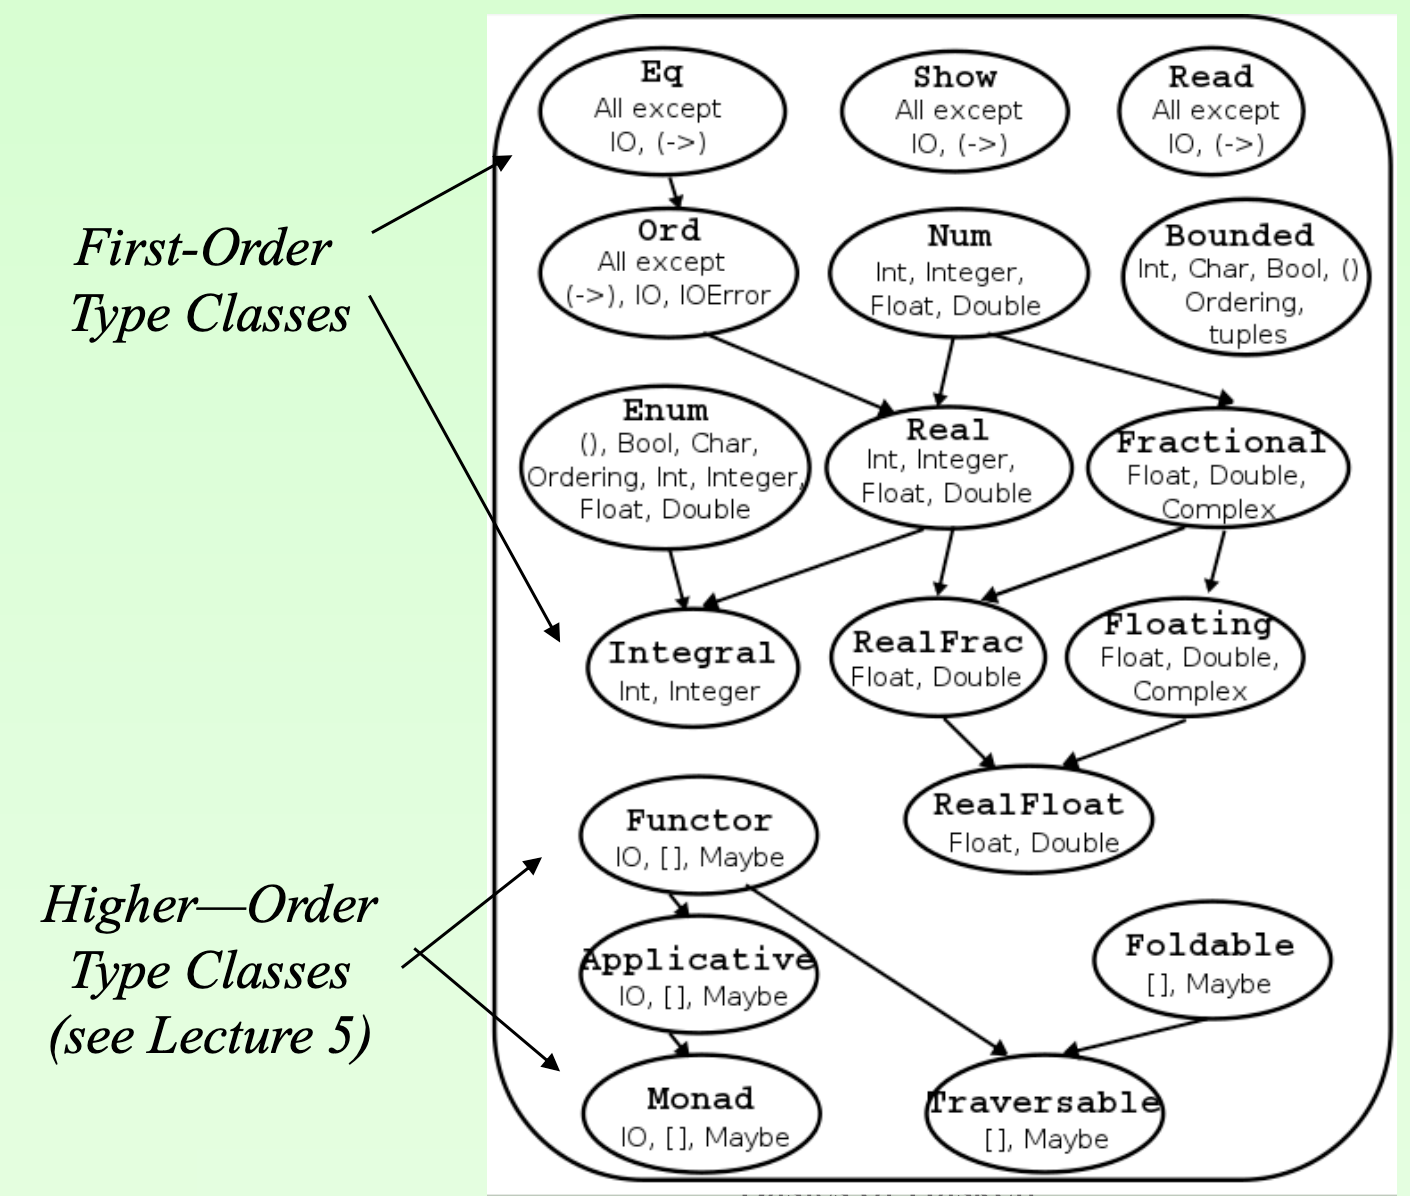
\includegraphics[width=\columnwidth]{L3/predefined-type-classes}
    \vspace{-0.3cm}
\section*{Higher-order functions}
  \begin{itemize}[leftmargin=*]
    \item Like data structures, fns should be first class:
      \begin{itemize}[leftmargin=*]
        \item Has value and type
        \item Can be passed as arg, returned as result, constructed at run-time, stored in data structures
      \end{itemize}
    \item HO functions are useful in supporting: \\
      \begin{hlist}
        \item Code reuse
        \item Laziness
        \item Data abstraction
        \item Design patterns
      \end{hlist}
  \end{itemize}
  \subsection*{Lazy evaluation}
    \begin{itemize}[leftmargin=*]
      \item Default for Haskell
      \item Any expression \ic{e} can be abstracted into a function: \ic{\\() -> e}
      \item Called a closure when it is coupled with value environment of free vars of \ic{e}: \ic{(E, \\() -> e)}
      \item Allows handling of non-terminating code, as long as it is not evaluated by context, like infinite data structures such as \ic{ones = 1:ones}
    \end{itemize}
  \subsection*{Strict evaluation} \noindent
    Helps avoid using memory for building closures, if result is definitely needed, e.g. \ic{inc !y = y+1}
  \subsection*{Folding}
    \begin{itemize}[leftmargin=*]
      \item Implement generalized functions
      \item Haskell fold types expect a \ic{Foldable}
    \end{itemize}
    \begin{lstlisting}
foldl :: Foldable t => (b -> a -> b) -> b -> t a -> b
foldr :: Foldable t => (a -> b -> b) -> b -> t a -> b
    \end{lstlisting}
    \begin{itemize}[leftmargin=*]
      \item Example impl below only support lists
      \item \ic{foldr} process from R to L, not tail-recursive
    \end{itemize}
    \begin{lstlisting}
foldr :: (a -> z -> z) -> z -> [a] -> z
foldr f z [] = z
foldr f z (x:xs) = f x (foldr f z xs)
-- Usage
sum xs = foldr (+) 0 xs
prod xs = foldr (*) 1 xs
    \end{lstlisting}
    \begin{itemize}[leftmargin=*]
      \item \ic{foldl} process from L to R, is tail-recursive
    \end{itemize}
    \begin{lstlisting}
foldl :: (z -> a -> z) -> z -> [a] -> z
foldl f z [] = z
foldl f z (x:xs) = foldl f (f z x) xs
    \end{lstlisting}
    \subsubsection*{Which to use}
      \begin{itemize}[leftmargin=*]
        \item Can be interchanged if reduction operator $f$ is associative
        \item \ic{foldl} typically more efficient due to tail recursion
      \end{itemize}
  \subsection*{List mapping}
    \begin{lstlisting}
map :: (a -> b) -> [a] -> [b]
map f [] = []
map f (x:xs) = (f x):(map f xs)
    \end{lstlisting}
  \subsection*{List filter}
    \begin{lstlisting}
filter :: (a -> Bool) -> [a] -> [a]
filter f [] = []
filter f (x:xs) =
  if (f x) then x:(filter f xs)
  else filter f xs
    \end{lstlisting}
  \subsection*{Mutual recursion} \noindent
    Mutual-recursive functions supported by multiple declarations within a single let construct
    \begin{lstlisting}
f n = 
  let foo n =
        if n <= 1 then 1
        else foo(n-1) + goo(n-2)
      goo n =
        if n <= 1 then 1
        else goo(n-1) + foo(n-2)
  in foo n
    \end{lstlisting}
  \subsection*{Function composition}
    \subsubsection*{Summary}
      \begin{lstlisting}
f (g x)      -- use space
(f . g) x    -- composition (R-to-L)
x |> g |> f  -- pipeline (left-to-right)
f $ g x      -- weak precedent apply
      \end{lstlisting}
    \subsubsection*{Types}
      \begin{lstlisting}
-- Regular function composition
(.) :: (b -> c) -> (a -> b) -> a -> c
(.) f g x = f (g x)
-- Left assoc
(|>) :: a -> (a -> b) -> b
a |> f = f a
-- Right assoc, low precedence
($) :: (a -> b) -> a -> b
f $ x = f x
-- Usage of weak precedent apply
inc $ x*2 <-> inc (x*2)
inc x*2 <-> (inc x)*2
      \end{lstlisting}
  \subsection*{List comprehension}
    \begin{itemize}[leftmargin=*]
      \item Equivalence with map:
    \end{itemize}
        \ic{[f x | x<-xs]} $\equiv$ \ic{map (\\x -> f x)} \ic{xs}
    \begin{itemize}[leftmargin=*]
      \item Supports filtering:
    \end{itemize}
        \ic{[f x | x<-xs, x>5]} $\equiv$ \\
        \ic{map (\\x -> f x)} \ic{(filter (\\x -> x>5)} \ic{xs)}
    \begin{itemize}[leftmargin=*]
      \item Can have multiple generators:
    \end{itemize}
        \ic{[(x,y) | x<-xs, y<-ys]} $\equiv$ \\
        \ic{concatMap (\\x -> map (\\y -> (x,y))} \ic{ys) xs)}
    \subsubsection*{General translation scheme}
      \begin{itemize}[leftmargin=*]
        \item \ic{[e | x<-xs]} $\equiv$ \ic{map (\x -> e) xs}
        \item \ic{[e | x<-xs, y<-ys, rest]} $\equiv$ \\
          \ic{concatMap (\x\ -> [e | y<-ys, rest])} \ic{xs}
        \item \ic{[e | x<-xs, test, rest]} $\equiv$ \\
          \ic{[e | x <- filter (\x\ -> test)} \ic{xs, rest]}
      \end{itemize}
    \subsubsection*{concatMap}
      \begin{lstlisting}
concatMap :: (a->b) -> [[a]] -> [b]
concatMap f [] = []
concatMap f (x:xs) = (f x) ++ (concatMap f xs)
      \end{lstlisting}
  \subsection*{Summary on Types/Expr}
    \begin{itemize}[leftmargin=*]
      \item Each type belongs to a kind -  \ic{type :: kind}
      \item Each type has \ic{*} as its kind, e.g. \ic{Int :: *}
      \item Type constructors are HO-functions over types, e.g.
        \begin{lstlisting}
Pair :: * -> * -> *
Pair Int :: * -> *
        \end{lstlisting}
      \item Three levels of typings - \ic{expr::type::kind}
        \begin{itemize}[leftmargin=*]
          \item Allows more type-safe expressions and kind-safe types to be safely constructed
        \end{itemize}
    \end{itemize}
  \subsection*{Arrays}
    \begin{itemize}[leftmargin=*]
      \item Use \ic{import Data.Array} to access
      \item \ic{Ix a =>} \ic{Array a b}
      \item Can be regarded as fns from indices to values, where indices are contiguous and bounded
      \item Array index up to a 5-tuple
      \item Cannot be infinite
    \end{itemize}
    \begin{lstlisting}
type Ix :: * -> Constraint
class (Ord a) => Ix a where
  range   :: (a,a) -> [a]
  inRange :: (a,a) -> a -> Bool
  index   :: (a,a) -> a -> Int
    \end{lstlisting}
    \begin{itemize}[leftmargin=*]
      \item \ic{range} enumerates a list of idx in index order
      \item \ic{inRange} checks if an index is between a pair of bounds
      \item \ic{index} gets zero-origin offset of an index from its bounds
    \end{itemize}
    \subsubsection*{Array creation}
      \begin{itemize}[leftmargin=*]
        \item Build using indices and a list of elements
        \item Can be defined recursively
      \end{itemize}
      \vspace{-0.1cm}
      \begin{lstlisting}
array :: (Ix a) => (a,a) -> [(a,b)] -> Array a b
-- Usage
squares = array (1,100) [(i, i*i) | i <- [1..100]]
squares ! 7 <=> 49
bounds squares <=> (1,100)
      \end{lstlisting}
    \subsubsection*{Accumulation}
      \begin{itemize}[leftmargin=*]
        \item Accumulate values into each index
        \item \ic{accumArray :: (Ix a)} \ic{=> (b->c->b)} \ic{-> b -> (a,a)} \ic{-> [Assoc a c] -> Array a b}
        \item Parameters are:
          \begin{hlist}
            \item accumulating function
            \item initial value
            \item bounds
            \item elements to accumulate
          \end{hlist}
      \end{itemize}
    \subsubsection*{Incremental updates}
      \begin{itemize}[leftmargin=*]
        \item \ic{(//) :: (Ix a)} \ic{=> Array a b -> [(a,b)] -> Array a b}
        \item e.g. \ic{a // [(i,v), (j,w)]}
        \item If an index appears multiple times, the last value takes precedence
      \end{itemize}
  \subsection*{Semi-group and monoids}
    \begin{lstlisting}
class SemiGroup a where
  op :: a -> a -> a
class SemiGroup a => Monoid a where
  unit :: a
    \end{lstlisting}
    \begin{itemize}[leftmargin=*]
      \item
        \begin{hlist}
          \item Associative
          \item Op with \ic{unit} returns itself
        \end{hlist}
      \item A monad is a higher-order monoid
    \end{itemize}
\section*{Monads}
  \subsection*{Referential transparency}
    \begin{itemize}[leftmargin=*]
      \item An expression is \textbf{referentially transparent} if it can be replaced with equivalent value (and vice versa) without changing the program's behavior/meaning
      \item Requires the expression to be pure
    \end{itemize}
  \subsection*{Summary}
    \begin{itemize}[leftmargin=*]
      \item Functors apply a function to a wrapped value
      \item Applicatives apply a wrapped function to a wrapped value
      \item Monads apply a function that returns a wrapped value, to a wrapped value
      \item Maybe implements all three
    \end{itemize}
  \subsection*{Contexts}
    \begin{itemize}[leftmargin=*]
      \item \ic{data Maybe a = Nothing | Just a}
      \item List \ic{[a]}:
        \begin{hlist}
          \item Empty list means no soln
          \item \ic{[r1,r2,r3]} means 3 possible solns
        \end{hlist}
      \item \ic{IO a} for input-output interaction
      \item \ic{DB a = state -> (state, a)} \\
        for imperative state that can be updated
      \item \ic{Parser a = String -> [(a,String)]} \\
        for non-deterministic parsing
    \end{itemize}
  \subsection*{Functor}
    \vspace{-0.2cm}
    \begin{lstlisting}
class Functor (f :: * -> *) where
  fmap :: (a -> b) -> f a -> f b
  -- replacing value in context with a
  (<$) :: a -> f b -> f a
  -- infix variant of fmap
  (<$>) :: (a -> b) -> f a -> f b
instance Functor Maybe where
  fmap f (Just val) = Just (f val)
  fmap f Nothing = Nothing
    \end{lstlisting}
    \vspace{-0.2cm}
  \subsection*{Applicative}
    \begin{itemize}[leftmargin=*]
      \item Can work with functions of any no. of args
    \end{itemize}
    \vspace{-0.2cm}
    \begin{lstlisting}
class Functor f => Applicative (f :: * -> *) where
  (<*>) :: f (a->b) -> f a -> f b
  -- takes a pure value and wraps it
  pure :: a -> f a
    \end{lstlisting}
    \vspace{-0.2cm}
  \subsection*{Monad}
    \vspace{-0.2cm}
    \begin{lstlisting}
class Monad m where
  -- bind operator
  >>= :: m a -> (a -> m b) -> m b
  return :: a -> m a
  >> :: (m a) -> (m b) -> m b
instance Monad Maybe where
  Nothing >>= f = Nothing
  Just val >>= f = f val
  m1 >> m2 = m1 >>= (\_ -> m2)
    \end{lstlisting}
    \subsubsection*{Monad laws}
      \vspace{-0.2cm}
      \begin{lstlisting}
-- Left identity
(return a) >>= k    = k a
-- Right identity
m >>= return        = m
-- Associativity
(m >>= f) >>= g     =
  m >>= (\x -> f x >>= g)
      \end{lstlisting}
    \subsubsection*{IO Monads}
      \vspace{-0.2cm}
      \begin{lstlisting}
getChar :: IO Char; getLine :: IO String
putChar :: Char -> IO ()
putStrLn :: String -> IO ()
readFile :: FilePath -> IO String
      \end{lstlisting}
  \subsection*{Do comprehension}
    \begin{itemize}[leftmargin=*]
      \item List is an instance of Monad; List comprehension is an instance of Do comprehension
      \item Every line is a monadic value, and can refer to computations in previous lines
      \item Using \ic{<-} lets us get the pure value, but cannot use for last line
      \item Each line of do comprehension is just a \ic{(>>=)}
    \end{itemize}
    \vspace{-0.2cm}
    \begin{lstlisting}
foo :: Maybe String  
foo = Just 3 >>= (\x -> Just "!" >>= (\y -> Just (show x ++ y)))
-- equivalent to
foo = do  
  x <- Just 3  
  y <- Just "!"  
  Just (show x ++ y)
    \end{lstlisting}
    \vspace{-0.2cm}
  \subsection*{Error handling}
    \vspace{-0.2cm}
    \begin{lstlisting}
-- using try-catch
class Monad m => MonadError e m | m -> e where
  throwError :: e -> m a
  catchError :: m a -> (e -> m a) -> m a
-- using Either
data Either a b = Left a | Right b
Left e   -- an error value of type a
Right x  -- a successful val x of type b
-- using Maybe
data Maybe a b = Nothing | Just b
Nothing   -- error value
Just x    -- success
    \end{lstlisting}
\end{multicols*}
\end{document}
